\documentclass[11pt,a4paper]{article}
\usepackage{amsmath}
\usepackage{amssymb}
\usepackage{graphicx}
\usepackage{verbatim}
\begin{document}
	\noindent
	Martin Lundfall, Henri Bunting, Malte Siemers, Patrik Bey
	\begin{centering}
		\section*{Exercise sheet 11 - Machine Intelligence I}
	\end{centering}
	\subsection*{11.1 - Cliques}
	In the given graph, we have 10 vertices and 17 edges. These make up 10 1-vertex cliques and 17 2-vertex cliques. We also identify the 3-vertex cliques consisting of vertices\\ $\{A,C,H\},\{A, C, G\},\{B, C, D\}, \{B, C, G\}, \{C, H, I\}, \{G, H, I\}$. There is also one 4-vertex clique, among the vertices $\{C, G, H, I\}$.
	\subsection*{11.2 - Cliques and Separators}
	\subsection*{(a)}
	The moralized graph of the DAG is an undirected graph where additional connections are added between nodes that share a child in the DAG.
	\begin{figure}[h]
		\caption{Moralization of the DAG}
		\centering
		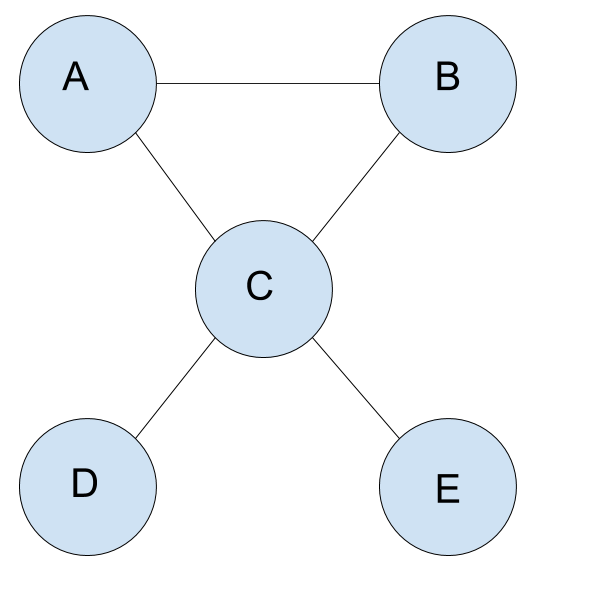
\includegraphics[width=.7\textwidth]{moral}
	\end{figure}
	\subsection*{(b)}
	Generally, the 1-vertex cliques are all the vertices of the moral graph, the 2-vertex cliques are formed by all the vertex pairs that are directly connected, and the only 3-vertex in the graph consists of $\{A, B C\}$. The separators of the graph are $\{C\}, \{A, C\}, \{B, C\}, \{C, D\}, \{C, E\}, \{A, B, C\}, \{A, C, E\},$\\$ \{A, C, D\}, \{B, C, D\}, \{B, C, E\}$.
	
	The given formula works only for maximal cliques and minimal separators. We have $\{A, B, C\}, \{B, C\}, \{C, E\}$ as a maximal cliques and $\{C\}$ as minimal separator.
	\begin{equation}
	\begin{split}
	p(a, b, c, d, e) = p(e|c)p(d|c)p(c|a,b)p(a,b) = \\
	\\
	= \frac{p(e, c)p(d, c)p(a, b, c)p(a, b)}{p(c)p(a, b)} = \frac{p(a, b, c)p(e, c)p(d, c)}{p(c)}
	\end{split}
	\end{equation}
	We see that in equation above the product of the cliques is the numerator and the separator is the denominator.
	
	\subsection*{11.3 Representation of the knowledge base}
	\subsubsection*{a)}
	\begin{verbatim}
	
	'''This is the burglary example from Exercise 10.3'''
	from bayesian.bbn import build_bbn
	
	def f_burglary(burglary):
	if burglary is True:
	return 0.01
	return 0.99
	
	def f_earthquake(earthquake):
	if earthquake is True:
	return 0.000001
	return 0.999999
	
	def f_radioBroadcast(earthquake, radioBroadcast):
	table = dict()
	table['tt'] = 1.
	table['tf'] = 0.
	table['ft'] = 0.
	table['ff'] = 1.
	key = ''
	key = key + 't' if earthquake else key + 'f'
	key = key + 't' if radioBroadcast else key + 'f'
	return table[key]
	\end{verbatim}
	\newpage
	\begin{verbatim}
	def f_alarm(burglary, earthquake, alarm):
	table = dict()
	table['fft'] = 0.001
	table['fff'] = 0.999
	table['ftt'] = 0.41
	table['ftf'] = 0.59
	table['tft'] = 0.95
	table['tff'] = 0.05
	table['ttt'] = 0.98
	table['ttf'] = 0.02
	key = ''
	key = key + 't' if burglary else key + 'f'
	key = key + 't' if earthquake else key + 'f'
	key = key + 't' if alarm else key + 'f'
	return table[key]
	
	if __name__ == '__main__':
	g = build_bbn(
	f_burglary,
	f_earthquake,
	f_radioBroadcast,
	f_alarm)
	g.q()
	\end{verbatim}
	\subsubsection*{b)}
	The code presented above creates the following output when run:
	\begin{verbatim}
	+----------------+-------+----------+
	| Node           | Value | Marginal |
	+----------------+-------+----------+
	| alarm          | False | 0.989510 |
	| alarm          | True  | 0.010490 |
	| burglary       | False | 0.990000 |
	| burglary       | True  | 0.010000 |
	| earthquake     | False | 0.999999 |
	| earthquake     | True  | 0.000001 |
	| radioBroadcast | False | 0.999999 |
	| radioBroadcast | True  | 0.000001 |
	+----------------+-------+----------+
	\end{verbatim}
	Here we can easily see the marginal probabilities $p(A = t) = 0.989510,$ \\$p(B = t) = 0.99, p(E = t) = 0.000001, p(R = t) = 0.000001$.
	This bayesian belief network uses a datastructure comprising four functions, one for each node in the DAG. For the independent events of a burglary and an earthquake occuring, we simply return the probability, whereas for the other nodes a probility is chosen from a table of probabilities depending on the input. When the \textit{Pythonic Bayesian Belief Network Framework} is built, it computes the marginal probabilities.
	
	\subsection*{11.4 - Potential Functions}
	\subsubsection*{(a)}
	%\emph{What are potential functions and what is the clique-marginal representation?}
	The potential function $a(C)$ for a given clique $C \in \mathrm{C}$ represents the quantitative input of $C$ to the probabilistic model. In the case of a directed acyclic graph it can be interpreted as the conditional distribution of the given random variable $X$ at node $v \in V$ $p(x_{v}|x_{parent(v)})$ whose factorization makes up $x$ joint distribution $p(x)$. For the general case the joint distribution can be understood as the factorization of potential functions over the given cliques $p(x) = \prod_{C \in \mathrm{C}}a_{C}(x_{x})$. To modify the potential function to incorporate local information, or evidence $\epsilon$, it may be modified to represent the likelihood of a random variable $x$ given the evidence resulting in the marginal representation for every clique $C$ and separator $S$:\\
	$P(X_{v}) = \frac{\prod_{C \in \mathrm{C}}a_{C}(X_{C})}{\prod_{S \in \mathrm{S}}b_{S}(X_{S})}$.
	
	
	\subsubsection*{(b)}
	%\emph{How can they be exploited to make inferences for the knowledge base}
	The marginal representation can be marginalized for every given clique $C$. This means that for any random variable the marginal probability can be computed individually and therefore reveal information about the knowledge base of the expert system, representing distribution of true diseases or similar features of the given expert system.
	
	\subsubsection*{(c)}
	%\emph{What is the benefit in comparison to the factorisation described in exercise 10.1?}
	The freedom in selection of the respective potential function allows for clique-wise individual representation of the probability density of the random variables contained in the respective clique, while holding a high level of generalization. This generalization is increased by the the concept of the  potential representation as the set of potential functions 
	$(\{a(C),C \in \mathrm{C}\},\{b(S),S \in \mathrm{S}\})$.
	
\end{document}
